\section{Near-cancelation of numbers}

In this section the computation of the function

\begin{align}
    f(x) = \frac{x+e^{-x}-1}{x^2}
\end{align}

should be analysed.

\subsection{Calculating the lim.}

First the limit $\lim_{x\to 0}f(x)$ should be calculated. This can easily be done with L'Hôpital's rule.
\begin{align}
\lim_{x\to 0}\frac{x+e^{-x}-1}{x^2} = \lim_{x\to 0} \frac{1-e^{-x}}{2x} = \lim_{x\to 0}\frac{1+e^{-x}}{2}=\frac{1}{2}   
\end{align}


\subsection{Interactive program to compute the function.}

The interactive program for the computation of this function is lokated
in the file \textit{part2.cpp}. For easy compilation
a \textit{CMakeLists.txt} file is included to use with \textit{cmake}.
The different parts of the program can be used by specifying different command line 
arguments. For the interactive program choose 0 and for the evaluation of the 
function for small values choose 1 as a command line argument.


\subsection{Analyse critical small values.}

If the function is evaluated for small values the formula goes wrong.
To determine the value of x for which this happens, the function
is evaluated for a range of small values and the results are plotted
in figure \ref{fig::f}.\\
It can be easily seen that for values of x arount $5\cdot 10^{-6}$ the formula
fails.

\begin{figure}[t]
    \centering
    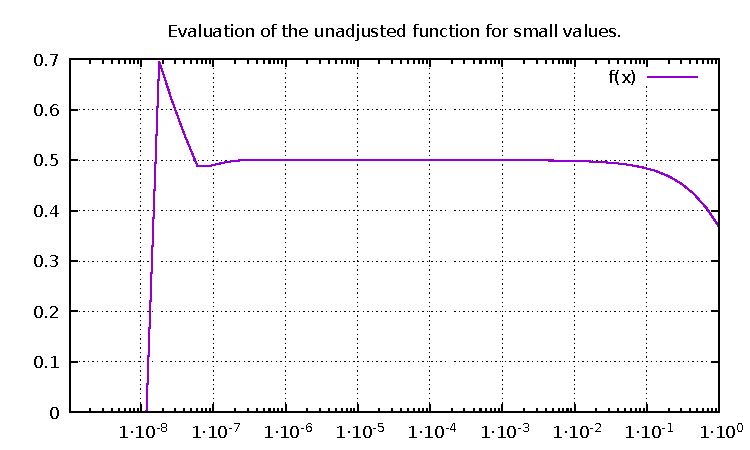
\includegraphics[width=0.8\textwidth]{../analysis/f.pdf}
    \caption{Evaluation of the function for small values.}
    \label{fig::f}
\end{figure}


\subsection{Explanation for the failure of the formula for small values}

From the taylor expansion it can be gathered that the second order term is the relevant term for small values of $x$. As such, given a mantissa of length $m$ and a precision $p$, the evaluation fails if
\begin{eqnarray}
    x^2 < 2^{-(m-p)}\\
    \Rightarrow x < 2^{-\frac{m-p}{2}}
\end{eqnarray}
since in those cases, $x^2$ cannot be reepresented to the given precision within the exponential function.\\
for a double ($m = 53$) with a precision of $p = 3$, this turns out to be
\begin{equation}
    x_{min} = 2^{-\frac{53 - 3}{2}} = 2^{-25} \approx 2.98\cdot 10^{-8}
\end{equation}

to get good values for the function, the third order term of the taylor expansion should also be included, which similarily breaks down at
\begin{equation}
    x_{min, err} = 2^{-\frac{m-p}{3}} \approx 9.61*10^{-6}
\end{equation}


\subsection{Adjustment for the calculation of the function.}

To get around the problem with the small values an if-statement can be
added to the execution of the function. This conditional case
will only be executed if the values of x are beneath the threshhold determined 
previously.\\
In order to get correct results for values beneath this threshhold
a different formular is needed. This can be done with the taylor
expansion of the function (1) which is given by:

\begin{align}
    f(x) = \sum_{n=0}^{\inf}\frac{(-x)^n}{(n+2)!}    
\end{align} 

Using the first three terms of this formular as an adustment to the function the overall 
results become reasonable. This is illustrated in figure \ref{fig::adjustedF}.

\begin{figure}[h]
    \centering
    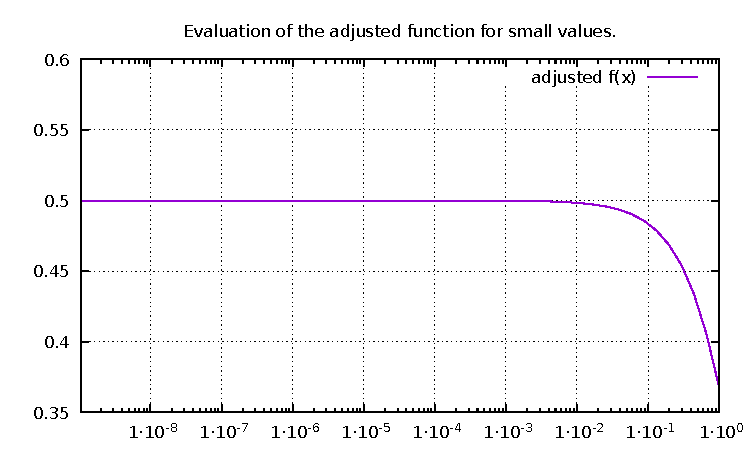
\includegraphics[width=0.8\textwidth]{../analysis/adjustedF.pdf}
    \caption{Evaluation of the adjusted function for small values.}
    \label{fig::adjustedF}
\end{figure}
